\section{Structure}

\subsection{Architecture}
\begin{figure}[hb]
    \centering
    \fbox{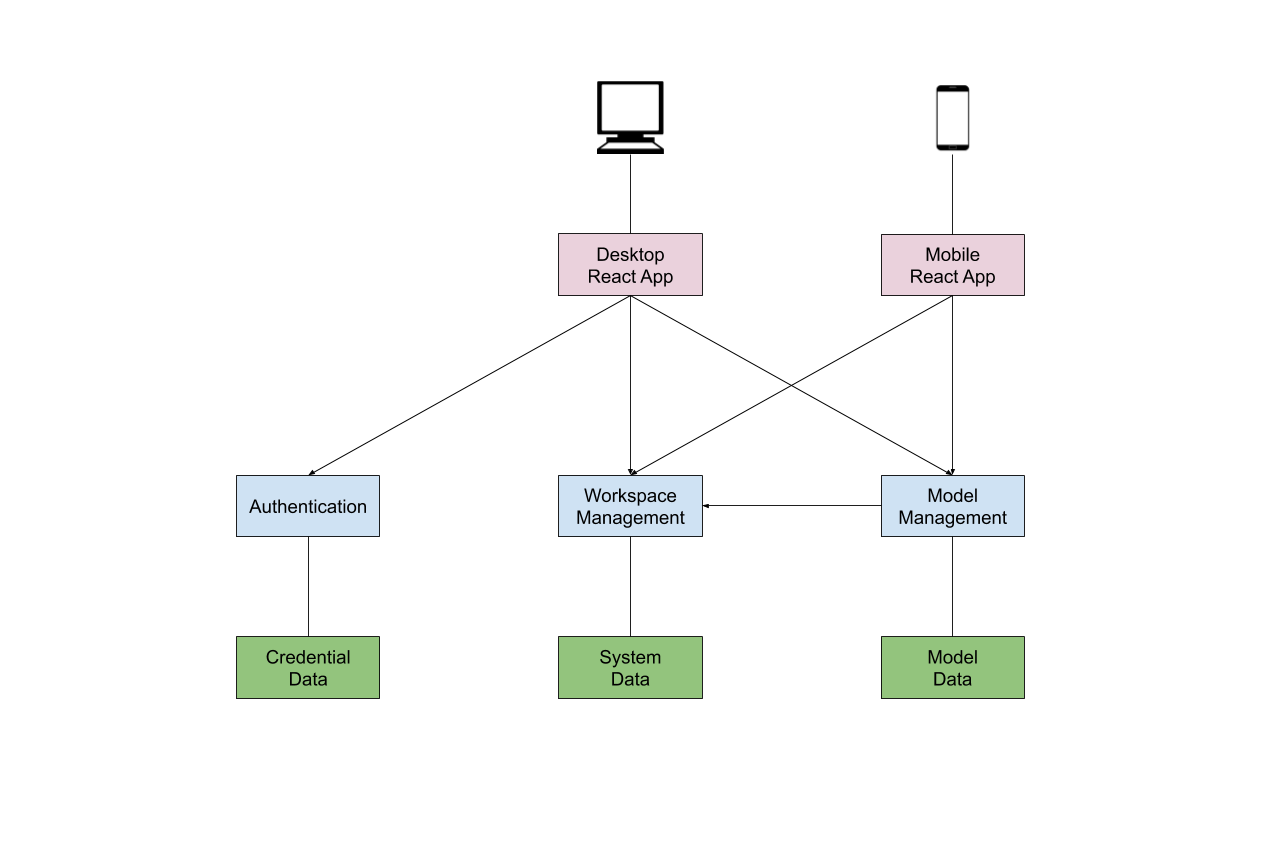
\includegraphics[width = .98\textwidth]{figures/architecture.png}}
    \caption{System Architecture as Microservices}
    \label{fig:microservices}
\end{figure}

General system architecture is designed according to the microservices architecture. Details of each microservice can be found below.

\subsection{Authentication}
Authentication service handles the registration of new users and authentication of registered users. The user registers by choosing a username, a password and supplying his email address. The authentication service then sends a verification token to this email address. The user creation is completed after the email verification.
\par The service uses JSON Web Tokens as the authentication method. After logging in, the user receives a cryptographically encrypted access token which is saved as a cookie. We encrypt the JWT that includes the username of the user and an expiration time (15 minutes after the creation) with a secret phrase that is shared among all the services that wish to use authentication. After receiving the access token with the requests, the services are able to decrypt the access token and verify the user identity. The user receives a refresh token in addition to the access token. This refresh token is used to renew an expired access token. This way, the user does not need to enter his credentials each time the token expires.

\subsection{Mobile and Desktop Clients}
Clients are implemented in a client-side-routed web app fashion using React and a routing library called raviger. All communication is routed through the API class, which, alongside dealing with authentication, acts as an adapter to the backend.
